\documentclass{report}

\input{~/dev/latex/template/preamble.tex}
\input{~/dev/latex/template/macros.tex}

\title{\Huge{Calculus 1 Chapter 5 Notes}}
\author{\huge{Nathan Warner}}
\date{\huge{April 21, 2023}}
\pagestyle{fancy}
\fancyhf{}
% \rhead{MATHEMATICS}
\rhead{MATHEMATICS}
% \chead{Chapter 5}
\lhead{Warner \thepage} 
\cfoot{\thepage}
% \usepackage[default]{sourcecodepro}
% \usepackage[T1]{fontenc}

\pgfpagesdeclarelayout{boxed}
{
  \edef\pgfpageoptionborder{0pt}
}
{
  \pgfpagesphysicalpageoptions
  {%
    logical pages=1,%
  }
  \pgfpageslogicalpageoptions{1}
  {
    border code=\pgfsetlinewidth{1.5pt}\pgfstroke,%
    border shrink=\pgfpageoptionborder,%
    resized width=.95\pgfphysicalwidth,%
    resized height=.95\pgfphysicalheight,%
    center=\pgfpoint{.5\pgfphysicalwidth}{.5\pgfphysicalheight}%
  }%
}

\pgfpagesuselayout{boxed}

\begin{document}
\maketitle
\begin{center}
  \begin{Huge}
    \textbf{Chapter 5}
  \end{Huge}
\end{center}
\line(1,0){490}
\bigbreak \noindent \bigbreak \noindent  
\begin{Huge}
  \noindent \textbf{Contents}
\end{Huge}
\bigbreak \noindent 
\begin{Large}
  \bigbreak \noindent
  \textbf{Review: Sigma Notation}
  \bigbreak \noindent \bigbreak \noindent 
  \textbf{5.1: Areas and Distances}
  \bigbreak \noindent \bigbreak \noindent 
  \textbf{5.2: The Definite Integral/Comparison Properties of the Integral Inequalities with Integrals}
  \bigbreak \noindent \bigbreak \noindent 
  \textbf{5.3: The Fundamental Theorem of Calculus}
  \bigbreak \noindent \bigbreak \noindent 
  \textbf{5.4: Indefinite Integrals and the Net Change Theorem}
  \bigbreak \noindent \bigbreak \noindent 
  \textbf{5.5: The Substitution Rule}
\end{Large}
\pagebreak \bigbreak \noindent

\pagebreak \bigbreak \noindent
\begin{Large}
  \begin{mdframed}
    \begin{center}
      \textbf{Review}
    \end{center}
  \end{mdframed}
\end{Large}
\begin{Large}
  \begin{center}
    \textbf{Sigma (Summation) Notation}
  \end{center}
\end{Large}
\line(1,0){490}

\bigbreak \noindent \bigbreak \noindent 
Sigma Notation is written like:
\begin{align*}
  \summation{n}{i=m}a^{i}
.\end{align*}
\bigbreak \noindent
Where $n$ is the number to stop the sum, and i=m tells us where to start our sum. $a_i$ is the general term.

\bigbreak \noindent 
Expanded sum:
\begin{align*}
  \summation{n}{i=m}a_i=a_m + a_{m+1} + a_{m+2} + ... + a_n
.\end{align*}

\bigbreak \noindent 
\nt{$i$ is called the \textbf{\textit{index of summation}}}

\bigbreak \noindent 
\begin{mdframed}
  \textbf{Properties:}
  \bigbreak \noindent 
  \begin{itemize}
    \item $\summation{n}{i=m}c \cdot a_i = c\summation{n}{i=m} a_{i}$, where c is a constant
    \item $\summation{n}{i=m} (a_{i} + b_{i})= \summation{n}{i=m} a_{i} + \summation{n}{i=m} b_{i} $
    \item $\summation{n}{i=m} (a_{i} - b_{i})= \summation{n}{i=m} a_{i} - \summation{n}{i=m} b_{i} $
    \item $\summation{n}{i=1} 1=n $
    \item $\summation{n}{i=1} c=c \cdot n $, where c is a constant
    \item $\summation{n}{i=1} i= \frac{n(n+1)}{2} $
    \item $\summation{n}{i=1}i^{2} = \frac{n(n+1)(2n+1)}{6} $
    \item $\summation{n}{i=1}i^{3}=\bigg[\frac{n(n+1)}{2}\bigg]^{2} $
  \end{itemize}
\end{mdframed}

\pagebreak \bigbreak \noindent
\begin{mdframed}
  \textbf{Example: Write in expanded form:}
  \begin{align*}
    \summation{5}{i=1}\sqrt{i}
  .\end{align*}
\end{mdframed}
\bigbreak \noindent
\textit{So:}
\begin{align*}
  \sqrt{1} + \sqrt{2} + \sqrt{3} + \sqrt{4} + \sqrt{5} \\
\end{align*}

\bigbreak \noindent 
\begin{mdframed}
  \textbf{Example: Write in sigma notation:}
  \begin{align*}
    1 + 2 + 4 + 8 + 16 + 32   
  .\end{align*}
\end{mdframed}

\bigbreak \noindent
\textit{So:}
\begin{align*}
  \summation{6}{i=0}2^{i}\ or\ \summation{6}{i=1}2^{i-1}
\end{align*}

\bigbreak \noindent 
\begin{mdframed}
  \textbf{Example: Write in expanded form:}
  \begin{align*}
    \summation{4}{k=0}\frac{2k-1}{2k+1}
  .\end{align*} 
\end{mdframed}

\bigbreak \noindent
\textit{So:}
\begin{align*}
  \frac{0-1}{0+1} +\frac{2-1}{2+1} +\frac{4-1}{4+1} +\frac{6-1}{6+1} +\frac{8-1}{8+1}  \\
  = -1 + \frac{1}{3} + \frac{3}{5} + \frac{5}{7} + \frac{7}{9} 
\end{align*}

\bigbreak \noindent 
\begin{mdframed}
  \textbf{Example: Find the value of the sum:}
  \begin{align*}
    \summation{n}{i=1}(i^{3}-i-2)   
  .\end{align*}
\end{mdframed}

\bigbreak \noindent 
\textit{Using properties of summations we can rewrite as:}
\begin{align*}
  \summation{n}{i=1}i^{3} - \summation{n}{i=1}i - \summation{n}{i=1}2 \\
  = \bigg[\frac{n(n+1)}{2}\bigg]^{2} - \frac{n(n+1)}{2} - 2n \\
  = \frac{n^{2}(n+1)^{2}}{4}- \frac{n(n+1)}{2} - 2n \\
  =\frac{n^{2}(n+1)^{2}}{4} - \frac{2n(n+1)}{4} -\frac{8n}{4} \\
  =\frac{n^{2}(n^{2}+2n+1)-2n^{2}-2n-8n}{4} \\
  = \frac{n^{4}+2n^{3}+n^{2}-2n^{2}-10n}{4} \\
  = \frac{n^{4}+2n^{3}-n^{2}-10n}{4} \\
  \boxed{= \frac{n(n^{3}+2n^{2}-n-10)}{4}}
.\end{align*}

\bigbreak \noindent 
\begin{mdframed}
  \textbf{Example: Evaluate the telescoping sum}
  \begin{align*}
    \summation{n}{i=1}i^{4}-(i-1)^{4}
  .\end{align*}
\end{mdframed}

\bigbreak \noindent 
\textit{Start by expanding the sum and see what pattern emerges}
\bigbreak \noindent
\textit{So:}
\begin{align*}
  (i^{4}-0^{4}) + (2^{4}-1^{4}) +(3^{4}-2^{4}) + ...\ + [(n-2)^{4}-(n-3)^{4}] + [(n-1)^{4}-(n-2)^{4}] + [n^{4}-(n-1)^{4}]
\end{align*}

\bigbreak \noindent \bigbreak \noindent 
\textit{You can see that we have Evaluated the sum for the first 3 terms, as well as for the last 3, and if you look at the terms, you can see that most of them will end up being canceled except for $0^{4}$ in the beginning and
  $n^{4}$ at the end
}

\bigbreak \noindent 
\textit{So we are left with:}
\begin{align*}
  0 + n^{4}\\
  \boxed{n^{4}}
.\end{align*}

\nt{Most of the terms ended up canceling out or \textit{collapsing}, which is why it's called a \textbf{\textit{\underline{telescoping sum}}}, it's important
  to note that hoever many terms end up surviving in the beginning of the sum, will be matched at the end of the sum.
}

\pagebreak \bigbreak \noindent
\begin{mdframed}
  \textbf{Example: Evaluate the telescoping sum:}
  \begin{align*}
    \summation{99}{i=3}\ \ \bigg(\frac{1}{i} -\frac{1}{i+1}\bigg)
  .\end{align*} 
\end{mdframed}

\bigbreak \noindent
\textit{So:}
\begin{align*}
  \bigg(\frac{1}{3}-\frac{1}{4}\bigg) + \bigg(\frac{1}{4}-\frac{1}{5}\bigg) + \bigg(\frac{1}{5}-\frac{1}{6}\bigg) + ... + \bigg(\frac{1}{97} - \frac{1}{98}\bigg) + \bigg(\frac{1}{98} - \frac{1}{99}\bigg) + \bigg(\frac{1}{99} - \frac{1}{100}\bigg)
\end{align*}

\bigbreak \noindent 
\textit{Again you can see that most of the terms will end up canceling out except:}

\begin{align*}
  \frac{1}{3} -\frac{1}{100}  \\
  = \frac{100}{300} - \frac{3}{300} \\
  \boxed{= \frac{97}{300}} \\
.\end{align*}

\bigbreak \noindent 
\begin{mdframed}
  \textbf{Example: Find the limit}
  \begin{align*}
    \lim_{n \to \infty}{\summation{n}{i=1}\ \ \frac{1}{n}\bigg(\frac{i}{n}\bigg)^{2}}
  .\end{align*} 
\end{mdframed}

\bigbreak \noindent 
\textit{We will start by pulling out constants:}

\bigbreak \noindent
\textit{So:}
\begin{align*}
  \lim_{n \to \infty}{\frac{1}{n}\cdot \frac{1}{n^{2}} \summation{n}{i=1}\ \ i^{2}} 
\end{align*}

\bigbreak \noindent 
\textit{From here we can clean up the expression and replace $i^{2}$ with the property of summations}

\bigbreak \noindent
\textit{So:}
\begin{align*}
  \lim_{n \to \infty}{\frac{1}{n^{3}} \frac{n(n+1)(2n+1)}{6}} \\
  =\lim_{n \to \infty}{\frac{1}{n^{2}} \frac{(n+1)(2n+1)}{6}} \\
  = \lim_{n \to \infty}{\frac{2n^{2}+3n+1}{6n^{2}}}
\end{align*}

\bigbreak \noindent 
\textit{Since the degree of the numerator is equal to the degree of the denominator the limit is going to be the 
  ratio of the leading coefficients.
}

\bigbreak \noindent
\textit{So:}
\begin{align*}
  \frac{2}{6} \\
  \boxed{= \frac{1}{3}}
\end{align*}

\pagebreak \bigbreak \noindent
\begin{mdframed}
  \textbf{Example: Find the limit:}
  \begin{align*}
    \lim_{n \to \infty}{\summation{n}{i=1}\ \ \frac{2}{n}\bigg[\bigg(\frac{2i}{n}\bigg)^{3} + 5 \bigg(\frac{2i}{n}\bigg)\bigg]}       
  .\end{align*}
\end{mdframed}

\bigbreak \noindent 
\textit{So again we will start by pulling out constants:}

\bigbreak \noindent
\textit{So:}
\begin{align*}
  \lim_{n \to \infty}{\frac{2}{n} \cdot \summation{n}{i=1}\ \ \bigg[\bigg(\frac{2i}{n}\bigg)^{3} + 5 \bigg(\frac{2i}{n}\bigg)\bigg]}\\
  =\lim_{n \to \infty}{\frac{2}{n} \cdot \summation{n}{i=1}\ \ \bigg[\bigg(\frac{8i^{3}}{n^{3}}\bigg) + 5 \bigg(\frac{2i}{n}\bigg)\bigg]}\\
\end{align*}

\bigbreak \noindent 
\textit{From here we can factor out an $\frac{2}{n}$}
\begin{align*}
  =\lim_{n \to \infty}{\frac{2}{n} \cdot \frac{2}{n} \cdot \summation{n}{i=1}\ \ \bigg[\frac{4i^{3}}{n^{2}} + 5i \bigg]}\\
  =\lim_{n \to \infty}{\frac{4}{n^{2}} \bigg[\frac{4}{n^{2}} \summation{n}{i=1}\ \ i^{3} + 5\summation{n}{i=1}\ \ i \bigg]} \\
  = \lim_{n \to \infty}{ \frac{4}{n^{2}}\bigg[\frac{4}{n^{2}}\bigg(\bigg(\frac{n(n+1)}{2}\bigg)\bigg)^{2} + 5\bigg(\frac{n(n+1)}{2}\bigg)\bigg]} \\
  = \lim_{n \to \infty}{\frac{4}{n^{2}}\bigg[\frac{n(n+1)}{2}\bigg(\frac{4n(n+1)}{2n^{2}}\bigg)+5\bigg]} \\
  = \lim_{h \to \infty}{\frac{4}{n^{2}}\bigg(\frac{n(n+1)}{2}\bigg)\bigg(\frac{4n^{2}+4n+10n^{2}}{2n^{2}}\bigg)} \\
  = \lim_{n \to \infty}{\frac{(n+1)(14n^{2}+4n)}{n^{3}}} \\
  = \lim_{n \to \infty}{\frac{14n^{3}+18n^{2} + 4n}{n^{3}}}
.\end{align*}

\bigbreak \noindent 
\textit{Again, since the degree of the numerator is equal to the degree of the denominator, we 
  take the ration of the leading coefficients to evaluate the limit.
}

\bigbreak \noindent
\textit{So:}
\begin{align*}
  \frac{14}{1} \\
  \boxed{=14}
\end{align*}

\pagebreak \bigbreak \noindent
\begin{Large}
  \begin{mdframed}
    \begin{center}
      \textbf{5.1}
    \end{center}
  \end{mdframed}
\end{Large}
\begin{Large}
  \begin{center}
    \textbf{Areas and Distances}
  \end{center}
\end{Large}
\line(1,0){490}

\bigbreak \noindent \bigbreak \noindent 
\begin{large}
  \textbf{The Area Problem}
\end{large}

\bigbreak \noindent 
\begin{figure}[ht]
    \centering
    \incfig{curve1}
    \label{fig:curve1}
\end{figure}
% \begin{center}
%   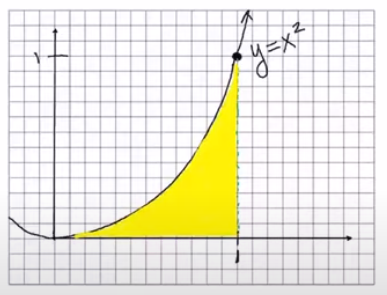
\includegraphics[scale=0.8]{ ./figures/1.png }
% \end{center}

\bigbreak \noindent 
Find the shaded area.
\bigbreak \noindent 
We dan't have an exact formula to compute, so we'll use approximation.

\bigbreak \noindent 
\textbf{\textit{\underline{Process.}}}
\smallbreak \noindent \smallbreak \noindent
We'll use rectangles to estimate the area.

\bigbreak \noindent 
\begin{figure}[ht]
    \centering
    \incfig{curve2}
    \label{fig:curve2}
\end{figure}
% \begin{center}
%   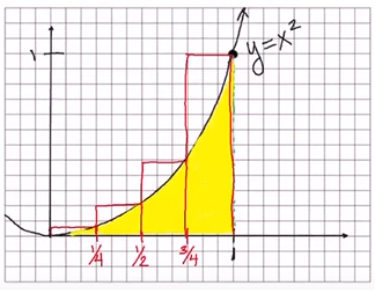
\includegraphics[scale=0.8]{ ./figures/2.png }
% \end{center}

\bigbreak \noindent 
Using right endpoints, we draw 4 rectangles:
\begin{itemize}
  \item $A_{1} = (\frac{1}{4})(\frac{1}{4})^{2} = \frac{1}{64} $
  \item $A_{2} =  (\frac{1}{4})(\frac{1}{2})^{2} = \frac{1}{16}$
  \item $A_{3} =  (\frac{1}{4})(\frac{3}{4})^{2} = \frac{9}{64}$
  \item $A_{4} =  (\frac{1}{4})(1)^{2} = \frac{1}{4}$
\end{itemize}
\bigbreak \noindent 
\nt{
  We find height by pulling x into the formula for the graph, ($x^{2}$)
}
\bigbreak \noindent 
Let $r_{4} = A_{1} + A_{2} + A_{3} + A_{4} = \frac{15}{32}$
\bigbreak \noindent 
So we can say the shaded region is $<$ $R_4$

\bigbreak \noindent \bigbreak \noindent 
Similarly, we form 4 rectangles using left endpoints.

\begin{figure}[ht]
    \centering
    \incfig{curve3}
    \label{fig:curve3}
\end{figure}
% \begin{center}
%   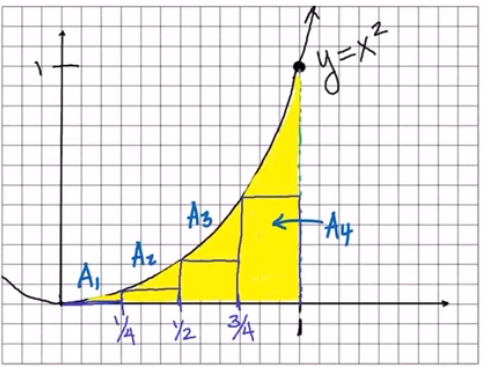
\includegraphics[scale=0.7]{ ./figures/3.png}
% \end{center}

\bigbreak \noindent 
\begin{itemize}
  \item $A_{1} = (\frac{1}{4})(0)^{2} = 0$
  \item $A_{2} = (\frac{1}{4})(\frac{1}{4})^{2} = \frac{1}{64} $
  \item $A_{3} =  (\frac{1}{4})(\frac{1}{2})^{2} = \frac{1}{16}$
  \item $A_{4} = (\frac{1}{4})(\frac{3}{4})^{2}  = \frac{9}{64}$
\end{itemize}
\bigbreak \noindent 
Let $L_{4} = A_{1} +A_{2} +A_{3} +A_{4} = \frac{7}{32}$

\bigbreak \noindent 
So we can say the shaded region $> L_{4} $

\bigbreak \noindent 
Now we have:
\begin{align*}
  L_{4} < A < R_{4}
.\end{align*}

\bigbreak \noindent 
We can improve the estimation by increasing the nmuber of rectangles. Therefore: 
\begin{align*}
  A \approx 0.33
.\end{align*}

\pagebreak \bigbreak \noindent
\begin{mdframed}
  \textbf{Example: Estimate the area under the graph of $f(x) = \cos{x}$ from $ x=0 $ to $x = \frac{\pi }{2} $ using 4 rectangles}
  \begin{itemize}
    \item a.) Right endpoints
    \item b.) Left endpoints
    \item c.) Which is an understimate/overestimate
  \end{itemize}
\end{mdframed}

\bigbreak \noindent 
\begin{figure}[ht]
    \centering
    \incfig{graph1}
    \label{fig:graph1}
\end{figure}
% \begin{center}
%   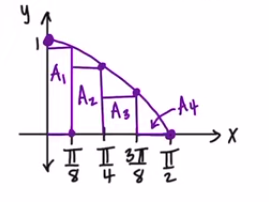
\includegraphics[scale=1]{ ./figures/4.png }
% \end{center}

\begin{align*}
  R_{4} = \frac{\pi}{8}(\cos{\frac{\pi }{8}} + \cos{\frac{\pi}{4}} + \cos{\frac{3\pi}{8}} + \cos{\frac{\pi}{2}}) \\
  \approx 0.7908  \\
  \boxed{underestimate}
.\end{align*}

\bigbreak \noindent 
\begin{figure}[ht]
    \centering
    \incfig{grahp2}
    \label{fig:grahp2}
\end{figure}
% \begin{center}
%   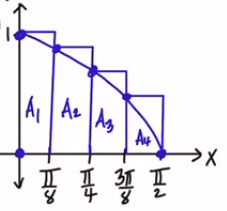
\includegraphics[scale=0.9]{ ./figures/5.png}
% \end{center}

\begin{align*}
  L_{4} = \frac{\pi}{8}(\cos{0} + \cos{\frac{\pi }{8}} + \cos{\frac{3\pi }{8}} + \cos{\frac{\pi }{2}})   \\
  \approx 1.1835 \\
  \boxed{overestimate}
.\end{align*}

\bigbreak \noindent \bigbreak \noindent
Now we'll use a formula for $n$ number of rectangles:

\bigbreak \noindent 
\begin{figure}[ht]
    \centering
    \incfig{curve5}
    \label{fig:curve5}
\end{figure}
% \begin{center}
%   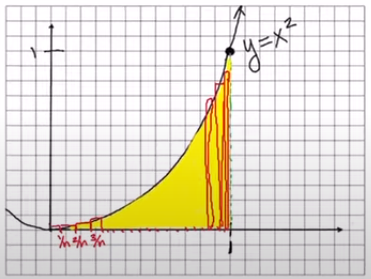
\includegraphics[scale=0.7]{./figures/6.png}
% \end{center}

\bigbreak \noindent 
In the previous $x^{2}$ example, we found the length of the base given the interval $[0,1]$ by:
\begin{align*}
  \frac{1-0}{4} = \frac{1}{4}
.\end{align*}

\bigbreak \noindent 
Now that we have $n$ rectangles, each rectangle has widith $\frac{1-0}{n}$ and height $\bigg(\frac{1}{n}\bigg)^{2},\ \bigg(\frac{2}{n}\bigg)^{2}$...

\bigbreak \noindent
\textit{So:}
\begin{align*}
  R_{n} = \frac{1}{n}\bigg(\frac{1}{n}\bigg)^{2} + \frac{1}{n} \bigg(\frac{2}{n}\bigg)^{2} + \frac{1}{n}\bigg(\frac{3}{n}\bigg)^{2} + ... + \frac{1}{n}\bigg(\frac{n}{n}\bigg)^{2} \\
  = \frac{1}{n}\bigg(\frac{1}{n^{2}} + \frac{2^{2}}{n^{2}}+\frac{3^{3}}{n^{2}} + ... + \frac{n^{2}}{n^{2}}\bigg) \\
  = \frac{1}{n} \cdot \frac{1}{n^{2}}(1+2^{2}+3^{2}+ ... + n^{2}) \\
  = \frac{1}{n^{3}} \bigg(\frac{n(n+1)(2n+1)}{6}\bigg) \\
  = \frac{n(n+1)(2n+1)}{6n^{2}}
\end{align*}

\bigbreak \noindent 
\textit{And:}
\begin{align*}
  \lim_{n \to \infty}{R_{n}=  \frac{2n^{2}+3n+1}{6n^{2}}} \\
  = \frac{2}{6} \\
  = \frac{1}{3}
.\end{align*}

\bigbreak \noindent 
Similarly, we can show that:
\begin{align*}
  \lim_{n \to \infty}{L_{n} = \frac{1}{3}}
.\end{align*}

\bigbreak \noindent 
Therefore: 
\begin{align*}
  A= \lim_{n \to \infty}{R_{n}} = \lim_{n \to \infty}{L_{n}} = \frac{1}{3}
.\end{align*}

\bigbreak \noindent \bigbreak \noindent 
\begin{mdframed}
  \textbf{Definition:}
  \bigbreak \noindent 
  The area under the graph of a continuous function $f(x)$ is:
  \begin{align*}
    A = \lim_{n \to \infty}{R_{n}} = \lim_{n \to \infty}{[\Delta xf(x_{1}) + \Delta xf(x_{2}) + ... + \Delta xf(x_{n})]}
  .\end{align*}
  \begin{center}
    or
  \end{center}
  \begin{align*}
    A = \lim_{n \to \infty}{L_{n}} = \lim_{n \to \infty}{[\Delta xf(x_{0}) + \Delta xf(x_{1}) + ... + \Delta xf(x_{n-1})]}
  .\end{align*}
  \begin{center}
    or
  \end{center}
  \begin{align*}
    A = \lim_{n \to \infty}{[\Delta xf(x_{1}^{*}) + ... + \Delta xf(x_{n}^{*})]}
  .\end{align*}
  \bigbreak \noindent 
  Where $x_{i}^{*}$ is any number in the $i$th interval.
  \nt{$\Delta x =$ Base of each rectangle
    \bigbreak \noindent 
    Find $\Delta x$ with $\frac{b-a}{n}$, on [a,b]
  }

  \bigbreak \noindent 
  Using $\summation{}{}$ "Sigma" notation, we have:
  \begin{itemize}
    \item $A = \lim\limits_{n \to \infty}{\summation{n}{i=1}\ \ \Delta xf(x_{i})} $ (Right endpoints)
    \item $A = \lim\limits_{n \to \infty}{\summation{n}{i=1}\ \ \Delta xf(x_{i-1})} $ (Left endpoints)
    \item $A = \lim\limits_{n \to \infty}{\summation{n}{i=1}\ \ \Delta xf(x_{i}^{*})} $ (Arbitrary partiton)
  \end{itemize}
  \bigbreak \noindent 
  \nt{The one with the star denotes not using left or right endpoints}
  \bigbreak \noindent 
\end{mdframed}

\bigbreak \noindent 
\begin{mdframed}
  \textbf{Example: Find an expression for the area under the graph of $f$ as a limit.}
  \begin{align*}
    f(x) = x^{2}+ \sqrt{1+2x},\ 3\leq x \leq 10
  .\end{align*}
\end{mdframed}

\bigbreak \noindent 
\textit{We need:}
\begin{align*}
  \Delta x = \frac{b-a}{n} \\
  = \frac{10-3}{n} \\
  = \frac{7}{n}
.\end{align*}

\bigbreak \noindent \bigbreak \noindent 
\textit{Now we need a formula for $x_{i}$, if we draw a number line:}

\bigbreak \noindent 
\begin{figure}[ht]
  \centering
  \incfig{deltax}
  \label{fig:deltax}
\end{figure}
% \begin{center}
%   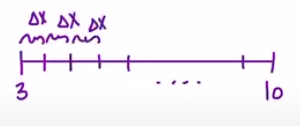
\includegraphics[scale=0.8]{ ./figures/7.png}
% \end{center}

\bigbreak \noindent 
\textit{We can see that:}
\begin{align*}
  x_{1} = 3 + \Delta x
.\end{align*}
\bigbreak \noindent 
\textit{And:}
\begin{align*}
  x_{2} = 3 + 2\Delta x
.\end{align*}

\bigbreak \noindent 
\textit{So we can see that the general formula for $x_{i}$ would be:}
\begin{align*}
  x_{i} = a + i \Delta x
.\end{align*}

\bigbreak \noindent 
\textit{So our $x_{i}$ is:}
\begin{align*}
  x_{i} = 3 + i \cdot \frac{7}{n} \\
  = 3 + \frac{7i}{n}
.\end{align*}

\bigbreak \noindent 
\textit{Now substitute $x_{i}$ into the function}

\bigbreak \noindent
\textit{So:}
\begin{align*}
  f(x_{i}) = \bigg(3+\frac{7i}{n}\bigg)^{2} + \sqrt{1+ 2\bigg(3 + \frac{7i}{n}\bigg)}
\end{align*}

\bigbreak \noindent 
\textit{Put everything together:}
\begin{align*}
  A = \lim\limits_{n \to \infty}{\summation{n}{i=1}\ \ \bigg(\frac{7}{n}\bigg)\bigg[\bigg(3+\frac{7i}{n}\bigg)^{2} + \sqrt{7+\frac{14i}{n}}\ \bigg]}
.\end{align*}

\bigbreak \noindent 
\textit{Where:}
\begin{figure}[ht]
  \centering
  \incfig{figure1}
  \label{fig:figure1}
\end{figure}


\pagebreak \bigbreak \noindent
\pagebreak \bigbreak \noindent
\begin{Large}
  \begin{mdframed}
    \begin{center}
      \textbf{5.2}
    \end{center}
  \end{mdframed}
\end{Large}
\begin{Large}
  \begin{center}
    \textbf{The Definite Integral}
  \end{center}
\end{Large}
\line(1,0){490}

\bigbreak \noindent \bigbreak \noindent 
From 5.1, Definition 2 gave the following limit for computing exact areas under the graph of $f(x)$ on [a,b]:
\begin{align*}
  A = \lim\limits_{n \to \infty}{R_{n} = \lim\limits_{x \to \infty}{\summation{n}{i=1}\ \ \Delta x \cdot f(x_{i})}}
.\end{align*}

\bigbreak \noindent 
In 5.2, we give the above setup a name: \textbf{Definite Integral:}
\begin{align*}
  \int_{a}^{b}f(x)dx = \lim\limits_{n \to \infty}{\summation{n}{i=1}\ \ \Delta xf(x_{i}^{*})}
.\end{align*}
\bigbreak \noindent 
Provided the limit exists and $x_{i}^{*}$ is any point in each subinterval
\bigbreak \noindent 
This technique is called \textbf{integration}.
\bigbreak \noindent 
\bigbreak \noindent 
\begin{mdframed}
  \textbf{Terms:}
  \bigbreak \noindent 
  \begin{center}
    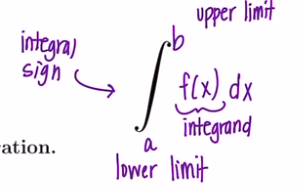
\includegraphics[scale=0.8]{./figures/8.png}
  \end{center}
\end{mdframed}

\bigbreak \noindent 
\nt{From definition 2:
  \begin{align*}
    A = \lim\limits_{x \to \infty}{\summation{n}{i=1}\ \ \Delta x \cdot f(x_{i})}        
  .\end{align*}
  \bigbreak \noindent 
  Just:
  \begin{align*}
    \summation{n}{i=1}\ \ \Delta xf(x_{i})
  .\end{align*}
  is called the \textbf{Rieman sum}
}

\bigbreak \noindent 
Also, if the regoin lies below the x-axis, its area will have a - sign

\bigbreak \noindent \bigbreak \noindent 
Example:
% \begin{figure}[ht]
%     \centering
%     \incfig{figure2}
%     \label{fig:figure2}
% \end{figure}

\begin{figure}[ht]
  \centering
  \incfig{aothuohu}
  \label{fig:aothuohu}
\end{figure}

\bigbreak \noindent 
\begin{mdframed}
  Properties of integrals:
  \begin{itemize}
    \item $\int_{a}^{b} cdx = c(b-a) $ 
    \item $\int_{a}^{b}cf(x)dx = c \cdot \int_{a}^{b}f(x)dx $
    \item $\int_{a}^{b}[f(x) + g(x)]dx = \int_{a}^{b}f(x)dx + \int_{a}^{b}g(x)dx$
    \item $\int_{a}^{b}[f(x) - g(x)]dx = \int_{a}^{b}f(x)dx - \int_{a}^{b}g(x)dx$
    \item $\int_{a}^{c}f(x)dx = \int_{a}^{b}f(x)dx + \int_{b}^{c}f(x)dx $
    \item if $f(x) \geq 0$ for all $a \leq x \leq b$, then $\int_{a}^{b}f(x)dx \geq  0 $
    \item if $f(x) \geq g(x) $ for all $a \leq x \leq b$, then $\int_{a}^{b}f(x)dx \geq \int_{a}^{b}g(x)dx $
    \item if $m \leq f(x) \leq M $ for $a \leq x \leq b$, then $m(b-a) \leq \int_{a}^{b}f(x)dx \leq M(b-a)$
  \end{itemize}
\end{mdframed}

\bigbreak \noindent 
\begin{mdframed}
  \textbf{Example: $f(x) = \sin{x},\ 0 \leq x \leq \frac{3\pi}{2} $}
  \bigbreak \noindent 
  Find the riemann sum with 6 terms, taking the sample points to be the right endpoints.
\end{mdframed}

\bigbreak \noindent 
\textit{First find $\Delta x$}
\bigbreak \noindent 
\textit{If:}
\begin{align*}
  \Delta x = \frac{b-a}{n}
.\end{align*}
\bigbreak \noindent 
\textit{Then:}
\begin{align*}
  \Delta x = \frac{\frac{3\pi}{2}-0}{6} \\
  = \frac{\pi}{4}
.\end{align*}

\bigbreak \noindent 
\textit{Next, find your 6 x values by adding $\frac{\pi}{4}$ to $\Delta x$}
\begin{align*}
  \bigg\{\frac{\pi}{4}, \frac{\pi}{2}, \frac{3\pi}{4}, \pi, \frac{5\pi}{4}, \frac{3\pi}{2} \bigg\} 
.\end{align*}

\bigbreak \noindent 
\textit{Now compute:}
\begin{align*}
  \Delta x \cdot (f(x_{1}) + f(x_{2}) + f(x_{3}) + f(x_{4}) + f(x_{5}) + f(x_{6}))
.\end{align*}

\bigbreak \noindent
\textit{So:}
\begin{align*}
  \frac{\pi }{4}\bigg(f\bigg(\frac{\pi}{4}\bigg) + f\bigg(\frac{\pi}{2}\bigg) + f\bigg(\frac{3\pi}{4}\bigg) + f\bigg(\pi\bigg) + f\bigg(\frac{5\pi}{4}\bigg)+ f\bigg(\frac{3\pi}{2}\bigg)\bigg) \\
  = \frac{\pi }{4}\bigg(\frac{\sqrt{2}}{2}\bigg) \\
  = \frac{\pi \sqrt{2}}{4} \\
  \boxed{\approx 0.5554}
\end{align*}

\bigbreak \noindent 
Repeat with midpoints as sample points:

\bigbreak \noindent 
\bigbreak \noindent 
\begin{figure}[ht]
  \centering
  \incfig{nmline}
  \label{fig:nmline}
\end{figure}
% \begin{center}
%   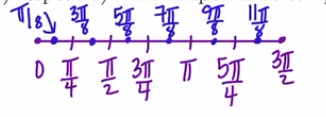
\includegraphics[scale=0.9]{ ./figures/9.png }
% \end{center}

\bigbreak \noindent 
\textit{Here we divided $\frac{\pi}{4}$ by 2 and added $\frac{\pi }{4}$ to each new subinterval to aquire our midpoints}

\bigbreak \noindent 
\nt{we can see that our $\Delta x$ is still $\frac{\pi}{4}$}

\bigbreak \noindent
\textit{So:}
\begin{align*}
  \frac{\pi}{4}\bigg(\sin{\frac{\pi}{8}} + \sin{\frac{3\pi}{8}} + \sin{\frac{5\pi}{8}} + \sin{\frac{7\pi}{8}} + \sin{\frac{9\pi}{8}} + \sin{\frac{11\pi}{8}}\bigg)  \\
  \boxed{\approx 1.0262}
\end{align*}

\bigbreak \noindent 
\begin{mdframed}
  \textbf{Example: Use midpoints with the given value of $n$ to approximate the integral}
  \begin{align*}
    \int_{2}^{10} \sqrt{x^{3} + 1}dx,\ n=4
  .\end{align*}
\end{mdframed}

\bigbreak \noindent
\textit{So:}
\begin{align*}
  a=2,\ b=10,\ f(x) = \sqrt{x^{3}+1},\ n=4
\end{align*}

\bigbreak \noindent 
\textit{Find $\Delta x$}
\begin{align*}
  \Delta x = \frac{10-2}{4} \\
  = 2
.\end{align*}

\bigbreak \noindent
\textit{Find midpoints:}
% \bigbreak \noindent 
% \begin{center}
%   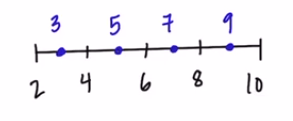
\includegraphics[scale=0.8]{ ./figures/10.png }
% \end{center}

\begin{figure}[ht]
  \centering
  \incfig{midpointfig}
  \label{fig:midpointfig}
\end{figure}

\bigbreak \noindent 
\textit{So:}
\begin{align*}
  A \approx \summation{4}{i=1}\ \ \Delta xf(x_{i})=
\end{align*}

\bigbreak \noindent 
\textit{Which is:}
\begin{align*}
  A \approx 2(f(3)+f(5)+f(7)+f(9)) \\
  \boxed{\approx 124.16}
.\end{align*}

\begin{mdframed}
  \textbf{Theorem 4:}
  \begin{align*}
    \int_{a}^{b}\ f(x)dx = \lim\limits_{x \to \infty}{\Delta x \cdot f(x_{i})}
  .\end{align*}
\end{mdframed}

\bigbreak \noindent 
\begin{mdframed}
  \textbf{Example: Evaluate using theorem 4:}
  \begin{align*}
    \int_{1}^{4}\ (x^{2} +2x-5)dx   
  .\end{align*}
  \bigbreak \noindent 
  Steps:
  \begin{enumerate}
    \item Find $\Delta x $
    \item Find $x_{i}$ ($a + i \cdot \Delta x $)
    \item Find $f(x_{i})$
  \end{enumerate}
\end{mdframed}

\bigbreak \noindent 
\textbf{1.)}
\begin{align*}
  \Delta x = \frac{4-1}{n} \\
  = \frac{3}{n}
.\end{align*}

\bigbreak \noindent 
\textbf{2.)}
\begin{align*}
  x_{i} = 1 + \frac{3i}{n}  \\
.\end{align*}

\bigbreak \noindent 
\textbf{3.) }
\begin{align*}
  f(x_{i}) = \bigg(1+\frac{3i}{n}\bigg)^{2} + 2\bigg(1+\frac{3i}{n}\bigg) -5
.\end{align*}

\bigbreak \noindent 
Now use the fact that:
\begin{align*}
  \int_{a}^{b}\ f(x)dx = \lim\limits_{x \to \infty}{\Delta x \cdot f(x_{i})}
.\end{align*}

\bigbreak \noindent
\textit{So:}
\begin{align*}
  \lim\limits_{n \to \infty}{\summation{n}{i=1}\ \ \bigg(\frac{3}{n}\bigg) \bigg[\bigg(1+\frac{3i}{n}\bigg)^{2} + 2\bigg(1+\frac{3i}{n}\bigg) -5\bigg]} \\
  = \lim\limits_{n \to \infty}{\frac{3}{n}\summation{n}{i=1}\ \ \bigg(1+\frac{6i}{n} + \frac{9i^{2}}{n^{2}} + 2 + \frac{6i}{n} -5\bigg)} \\
  = \lim\limits_{n \to \infty}{\frac{3}{n} \summation{n}{i=1}\ \ \bigg(\frac{9i^{2}}{n^{2}} + \frac{12i}{n} -2\bigg)}
\end{align*}

\bigbreak \noindent 
\textit{From here use properties of summation:}
\begin{align*}
  \lim\limits_{n \to \infty}{\frac{3}{n}\bigg[\summation{n}{i=1}\ \ \frac{9}{n}i^{2} + \summation{n}{i=1}\ \ \frac{12}{n}i - \summation{n}{i=1}\ \ 2\bigg]} \\
  = \lim\limits_{n \to \infty}{\frac{3}{n}\bigg[\frac{9}{n^{2}}\ \summation{n}{i=1} i^{2} + \frac{12}{n}\summation{n}{i=1} i - 2n \bigg]} \\
  = \lim\limits_{n \to \infty}{\frac{3}{n}\bigg[\frac{9}{n^{2}} \frac{n(n+1)(2n+1)}{6} + \frac{12}{n} \cdot \frac{n(n+1)}{2} -2n\bigg]}
.\end{align*}

\bigbreak \noindent 
Now using limit rules we have:
\begin{align*}
  \lim\limits_{n \to \infty}{\frac{9}{2}\frac{(n+1)(2n+1)}{n^{2}}} + \lim\limits_{n \to \infty}{\frac{18(n+1)}{n}} - \lim\limits_{n \to \infty}{6} \\
  = \lim\limits_{n \to \infty}{\frac{9}{2}\frac{(2n^{2} +3n+1)}{n^{2}}} + \lim\limits_{n \to \infty}{\frac{18n+18}{n}} - \lim\limits_{n \to \infty}{6} \\
  = \frac{9}{2} \cdot 2 + 18 - 6 \\
  \boxed{21}
.\end{align*}
\bigbreak \noindent 
\nt{Recall if the degree of the numerator is equal to the degree of the denominator we take the ratio of the leading terms}

\bigbreak \noindent 
\begin{mdframed}
  \textbf{Example: Evaluate in terms of areos. (Hint: Use Geometry!)}
  \begin{align*}
    \int_{-2}^{2}\ \sqrt{4-x^{2}}dx
  .\end{align*}
\end{mdframed}

\bigbreak \noindent
\textit{So:}
\begin{align*}
  f(x) = \sqrt{4-x^{2}}
\end{align*}

\bigbreak \noindent \bigbreak \noindent
\nt{This is an equation for a semicircle, because:
  \begin{align*}
    y = \sqrt{4-x^{2}} \\
    y^{2} = 4-x^{2} \\
    x^{2} + y^{2} = 4\ r=2
  .\end{align*}
  \bigbreak \noindent 
  We know it's only the upper half of the semicircle because we only have the positive version
}
% 
% \bigbreak \noindent 
% \textit{Figure:}
% \bigbreak \noindent 
% \begin{center}
%   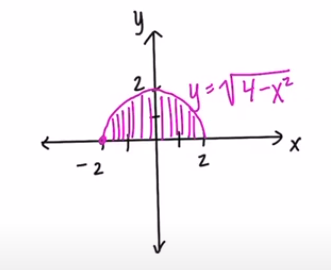
\includegraphics[scale=0.8]{ ./figures/11.png }
% \end{center}

\begin{figure}[ht]
  \centering
  \incfig{circlefig}
  \label{fig:circlefig}
\end{figure}

\bigbreak \noindent
\textit{So:}
\begin{align*}
  A = \frac{\pi r^{2}}{2 } \\
  = \frac{\pi(2)^{2}}{2} \\
  \boxed{= 2\pi}
\end{align*}

\bigbreak \noindent 
\begin{mdframed}
  \textbf{Example: Evaluate in terms of areas. (Hint: Use Geometry)}
  \begin{align*}
    \int_{-1}^{3}(3-2x)dx
  .\end{align*}
\end{mdframed}

\bigbreak \noindent
\textit{So:}
\begin{align*}
  f(x) = 3-2x
\end{align*}

\bigbreak \noindent 
\nt{This is an equation for a line ($y=mx+b$)}

\begin{align*}
  x-int:\ 0 = -2x+3 \\
  x=\frac{3}{2},\ so\ (\frac{3}{2}, 0)
.\end{align*}
\begin{align*}
  y-int:\ (0,3)
.\end{align*}

\bigbreak \noindent 
\textit{Evaluate at endpoints:}
\begin{align*}
  f(-1) = 5 \\
  f(3) = -3
.\end{align*}
%
% \bigbreak \noindent 
% \textit{Figure:}
% \bigbreak \noindent 
% \begin{center}
%   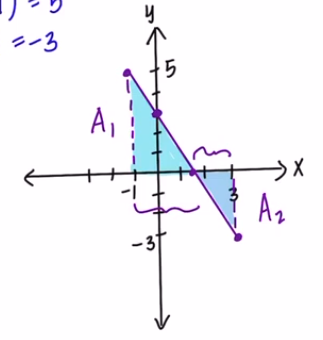
\includegraphics[scale=0.6]{ ./figures/12.png }
% \end{center}

\begin{figure}[ht]
  \centering
  \incfig{figure11}
  \label{fig:figure11}
\end{figure}



\bigbreak \noindent 
\textit{Notice we have 2 triangles, so find the area for each, ($A=\frac{1}{2}bh$)}

\begin{align*}
  A_{1} = \frac{1}{2}(2.5)(5) \\
  = 6.25 \\
  A_{2} = \frac{1}{2}(1.5)(3) \\ 
  = 2.25 \\
  Net\ Area\ =\ A_{1} - A_{2} \\
  \boxed{6.25 - 2.25 = 3.25}
.\end{align*}

\bigbreak \noindent 
\nt{We subtracted $A_{2}$ because $A_{2}$ was below the x axis therefore it is \textbf{\textit{negative area}}}

\pagebreak \bigbreak \noindent
\begin{mdframed}
  \begin{large}
    \begin{center}
      \textbf{Comparison Properties of the integral inequalities with integrals}
    \end{center}
  \end{large}
\end{mdframed}
\line(1,0){490}
\bigbreak \noindent \bigbreak
\begin{mdframed}
  \textbf{Properties:}
  \begin{enumerate}
    \item If $f(x) \geq 0$ for all $a \leq x \leq b  $, then $\int_{a}^{b}f(x)dx \geq 0$
    \item If $f(x) \geq g(x)$ for all $a \leq x \leq b $, then $\int_{a}^{b}f(x)dx \geq \int_{a}^{b}g(x)dx$
    \item if $m \leq f(x) \leq M$ for $a \leq x \leq b$, then
      \begin{align*}
        m(b-a) \leq \int_{a}^{b}f(x)dx \leq M(b-a)
      .\end{align*}
  \end{enumerate}
\end{mdframed}

\bigbreak \noindent 
\begin{mdframed}
  \textbf{Example: Use the properties of integrals to verify the inequality without evaluating the integrals.}
  \begin{align*}
    \int_{0}^{1}\ \sqrt{1+x^{2}}\ dx \leq \int_{0}^{1}\sqrt{1+x}\ dx
  .\end{align*}
\end{mdframed}

\bigbreak \noindent 
With \textbf{Property 2.}
\begin{align*}
  If\ f(x) \geq g(x)\ for\ all\ a \leq x \leq b,\ then\ \int_{a}^{b}f(x)\ dx \geq \int_{a}^{b}g(x)\ dx 
.\end{align*}

\bigbreak \noindent  \bigbreak \noindent 
On, the interval [0,1] We know
\begin{align*}
  x^{2} \leq x 
.\end{align*}

\bigbreak \noindent \bigbreak \noindent 
Therefore

\begin{align*}
  1+x^{2} \leq 1+ x \\
  so \\
  \sqrt{1+x^{2}} \leq \sqrt{1+x}\ on\ [0,1]
.\end{align*}

\bigbreak \noindent \bigbreak \noindent
Hence we have showed that 
\begin{align*}
  \int_{0}^{1}\ \sqrt{1+x^{2}}\ dx \leq \int_{0}^{1}\sqrt{1+x}\ dx 
.\end{align*}

\pagebreak \bigbreak \noindent
\bigbreak \noindent 
\begin{mdframed}
  \textbf{Example: }
  \begin{align*}
    2 \leq \int_{-1}^{1}\ \sqrt{1+x^{2}}\ dx \leq 2\sqrt{2}
  .\end{align*}
\end{mdframed}

\bigbreak \noindent \bigbreak \noindent
With property 3, which states:

\bigbreak \noindent \bigbreak \noindent
\begin{itemize}
  \item if $m \leq f(x) \leq M$ for $a \leq x \leq b$, then
\end{itemize}
\begin{align*}
  m(b-a) \leq \int_{a}^{b}f(x)dx \leq M(b-a)
.\end{align*}

\bigbreak \noindent \bigbreak \noindent
We know x has to obey
\begin{align*}
  x \in [-1,1] \\
  or \\
  -1 \leq x \leq 1
.\end{align*}

\bigbreak \noindent \bigbreak \noindent
Next we want to try to make the x in the inequality above become our function $\sqrt{1+x^{2}}$

\bigbreak \noindent \bigbreak \noindent
Step 1.) Square everything in the equality to get $x^{2}$
\begin{align*}
  0 \leq x^{2} \leq 1
.\end{align*}

\nt{
  Since we squared the inequality, all the negatives are gone, but zero remains. Therefore our inequality is now bounded between 0 and 1.
}

\bigbreak \noindent \bigbreak \noindent
Step 2.) Add one to the inequality.
\begin{align*}
  1 \leq 1+ x^{2} \leq 2
.\end{align*}

\bigbreak \noindent \bigbreak \noindent 
Step 3.) Take the square root of the inequality.
\begin{align*}
  1 \leq \sqrt{1+x^{2}} \leq \sqrt{2}
.\end{align*}

\bigbreak \noindent \bigbreak \noindent
Now we can apply the third comparison property.
\begin{align*}
  1(1-(-1)) \leq \int_{-1}^{1}\ \sqrt{1+x^{2}}\ dx \leq \sqrt{2}(1-(-1)) \\
  2 \leq \int_{-1}^{1}\ \sqrt{1+x^{2}}\ dx \leq 2\sqrt{2}
.\end{align*}

\pagebreak \bigbreak \noindent
\bigbreak \noindent 
\begin{mdframed}
  \textbf{Example: Use the comparison properties of integras to prove the inequality.}
  \begin{align*}
    \int_{1}^{3}\ \sqrt{x^{4} + 1}\ dx \geq \frac{26}{3} 
  .\end{align*}
\end{mdframed}

\bigbreak \noindent \bigbreak \noindent
Since our function is not easily integratable, we will show that it is greater than something we can easily integrate.

\begin{align*}
  \sqrt{x^{4} +1} \geq \sqrt{x^{4}} = x^{2}
.\end{align*}

\bigbreak \noindent
\textit{So:}
\begin{align*}
  \int_{1}^{3}\ \sqrt{x^{4} + 1}\ dx \geq \int_{1}^{3}x^{2}\ dx
\end{align*}

\bigbreak \noindent \bigbreak \noindent
Evaluate $\int_{1}^{3}\ x^{2}\ dx$ by finding the antiderivitive

\begin{align*}
\frac{1}{3}x^{3}\bigg]_{1}^{3} \\
= \frac{1}{3}(3^{3} -1^{3}) \\
\boxed{= \frac{26}{3}}
.\end{align*}

\bigbreak \noindent \bigbreak \noindent
Therefore we have shown that
\begin{align*}
  \int_{1}^{3}\ \sqrt{x^{4} + 1}\ dx \geq \frac{26}{3} 
.\end{align*}

\bigbreak \noindent 
\begin{mdframed}
  \textbf{Example}
  \begin{align*}
    \int_{0}^{\frac{\pi}{2}}\ x\sin{x}\ dx \leq \frac{\pi^{2}}{8}
  .\end{align*}
\end{mdframed}

\bigbreak \noindent \bigbreak \noindent
Let's try and bound our $f(x)$ above something we can easily integrate. We know $\sin{x}$ is bounded between -1 and 1, but in this case we are only looking at quadrant I. In this scenario $\sin{x}$ is bounded between 0 and 1.

\bigbreak \noindent \bigbreak \noindent
So.
\begin{align*}
  \sin{x} \leq 1\ if\ 0 \leq x \leq \frac{\pi}{2}
.\end{align*}

\bigbreak \noindent \bigbreak \noindent
Like the previous example, we want our inequality to involve our $f(x)$, so we multiply everything by x

\begin{align*}
  x\sin{x} \leq x
.\end{align*}

\pagebreak \bigbreak \noindent
Now we can integrate
\begin{align*}
  \int_{0}^{\frac{\pi}{2}}\ x\sin{x}\ dx \leq \int_{0}^{\frac{\pi}{2}}\ x\ dx
.\end{align*}

\bigbreak \noindent
So:
\begin{align*}
\frac{1}{2}x^{2}\bigg]_{0}^{\frac{\pi}{2}} \\
= \frac{1}{2}\bigg[\bigg(\frac{\pi}{2}\bigg)^{2} - 0^{2}\bigg] \\
\boxed{= \frac{\pi^{2}}{8}}
\end{align*}

\bigbreak \noindent 
\begin{mdframed}
  \textbf{Example: }
  \begin{align*}
    \int_{0}^{1}\ \sqrt{1+e^{2x}}\ dx \geq e-1
  .\end{align*}
\end{mdframed}

\begin{align*}
  \sqrt{1+e^{2x}} > \sqrt{e^{2x}} = e^{x} \\
  \sqrt{1+e^{x}} \geq e^{x} \\
.\end{align*}
\begin{align*}
  \int_{0}^{1}\ \sqrt{1+e^{x}}\ dx \geq \int_{0}^{1}e^{x}\ dx \\
= e^{x}\bigg]_{0}^{1} \\
= e^{1} - e^{0} \\
\boxed{= e-  1}
.\end{align*}

\bigbreak \noindent 
\begin{mdframed}
  \textbf{Example: }
  \begin{align*}
    \int_{0}^{1}\ e^{x}\cos{x}\ dx \leq e-1
  .\end{align*}
\end{mdframed}

\bigbreak \noindent \bigbreak \noindent
We know:
\begin{align*}
  \cos{x} \leq 1 \\
  and \\
  e^{x} > 0
.\end{align*}
\bigbreak \noindent \bigbreak \noindent
Therefore:
\begin{align*}
  e^{x}\cos{x} \leq e^{x}
.\end{align*}

\bigbreak \noindent
\textit{So:}
% \begin{align*}
%   \int_{0}^{1}e^{x}\cos{x}\ dx \leq \int_{0}^{1}e^{x}\ dx \\
%   = e^{x}\bigg]_{0}^{1} \\
% \boxed{e-1}
% \end{align*}

\pagebreak \bigbreak \noindent
\begin{Large}
  \begin{mdframed}
    \begin{center}
      \textbf{5.3}
    \end{center}
  \end{mdframed}
\end{Large}
\begin{Large}
  \begin{center}
    \textbf{The Fundamental Theorem of Calculus}
  \end{center}
\end{Large}
\line(1,0){490}

\bigbreak
\begin{mdframed}
  \textbf{Theorem:}
  \smallbreak \noindent \smallbreak \noindent
  If $f$ is continuous on [a,b], then:
  \begin{align*}
    Part\ 1:\ \frac{d}{dx}\int_{a}^{x}\ f(x)\ dt  = f(x), a \leq x \leq b         \\
    Part\ 2:\ \int_{a}^{b}\ f(x)\ dx = F(b) - F(a)\ where\ F^{\prime} = f.
  .\end{align*}
\end{mdframed}

\bigbreak \noindent 
\begin{mdframed}
  \textbf{Example: Use Part 1 of the Fundamental Theorem of calculus to find the derivative of the function}
  \begin{align*}
    g(x) = \int_{1}^{x}e^{t^{2} -t}\ dt
  .\end{align*}
  \bigbreak \noindent \bigbreak \noindent
  We will make use of the property:
  \begin{align*}
    \int_{a}^{b}\ f(x)\ dx = -\int_{b}^{a}\ f(x)\ dx
  .\end{align*}
\end{mdframed}
\bigbreak \noindent \bigbreak \noindent
So:
\begin{align*}
  g^{\prime}(x) = \frac{d}{dx}\int_{1}^{x}\ e^{t^{2}-t}\ dt
.\end{align*}

\bigbreak \noindent \bigbreak \noindent
Replace instances of t with x, because x is our upper limit.

\begin{align*}
  g^{\prime}(t) = \frac{d}{dx} \int_{1}^{x}\  = \boxed{e^{x^{2}-x}}
.\end{align*}

\bigbreak \noindent 
\begin{mdframed}
  \textbf{Example: }
  \begin{align*}
    g(t) = \int_{0}^{t}\ \sqrt{r^{2}+4}\ dx
  .\end{align*}
\end{mdframed}

\bigbreak \noindent \bigbreak \noindent
Replace instances of r with t
\begin{align*}
  g^{\prime}(t) = \frac{d}{dt}\ \int_{0}^{t}\ \sqrt{r^{2}+ 4}\ dr = \boxed{\sqrt{t^{2} + 4}}
.\end{align*}

\pagebreak \bigbreak \noindent
\bigbreak \noindent 
\begin{mdframed}
  \textbf{Example: }
  \begin{align*}
    G(x) = \int_{x}^{1}\ \cos{\sqrt{t}}\ dt
  .\end{align*}
\end{mdframed}

\bigbreak \noindent \bigbreak \noindent
Notice we cannot apply the Fundamental thoerem of calculus because our upper limit is not a constant, therefore we must utilize the property:
\begin{align*}
  \int_{a}^{b}\ f(x)\ dx = -\int_{b}^{a}\ f(x)\ dx
.\end{align*}

\bigbreak \noindent
So:
\begin{align*}
  -\int_{1}^{x}\ \cos{\sqrt{t}}\ dt  
\end{align*}

\bigbreak \noindent \bigbreak \noindent
Which means:
\begin{align*}
  \boxed{G^{\prime}(x) = -\cos{\sqrt{t}}\ dt}
.\end{align*}

\bigbreak \noindent 
\begin{mdframed}
  \textbf{Example: }
  \begin{align*}
    y = \int_{1}^{\cos{r}}\ (a+x^{2})^{10}\ dx
  .\end{align*}
\end{mdframed}

\bigbreak \noindent \bigbreak \noindent
Replace x with upper limit:
\begin{align*}
  y^{\prime} = (1+(\cos{r})^{2})^{10}\ \frac{d}{dr}(\cos{r}) \\
  = (1+\cos^{2}{r})^{10}(-\sin{r}) \\
  \boxed{= -\sin{r}(1+\cos^{2}{r})^{10}}
.\end{align*}

\bigbreak \noindent \bigbreak \noindent
\begin{mdframed}
  \textbf{Now let's look at part 2 of the Fundamental theorem of calculus.}
  \bigbreak \noindent 
  Which States:
  \begin{align*}
    \int_{a}^{b}\ f(x)\ dx = F(b) - F(a)\ where\ F^{\prime} = f
  .\end{align*}
\end{mdframed}

\pagebreak \bigbreak \noindent
\begin{mdframed}
  \textbf{Example: }
  \begin{align*}
    \int_{1}^{8}\ \sqrt[3]{x}\ dx
  .\end{align*} 
\end{mdframed}


\bigbreak \noindent
Find the antiderivitive
\begin{align*}
  \frac{x^{\frac{1}{3}+1}}{\frac{4}{3}} 
  = \frac{3}{4}x^{\frac{4}{3}}
\end{align*}

\bigbreak \noindent \bigbreak \noindent
Now 
\begin{align*}
\frac{3}{4}x^{\frac{4}{3}}\bigg]_{1}^{8}
.\end{align*}

\bigbreak \noindent \bigbreak \noindent
To evaluate, use 
\begin{align*}
  F(b) - f(a)
.\end{align*}

\bigbreak \noindent
So:
\begin{align*}
  \frac{3}{4}(8^{\frac{4}{3}} - 1^{\frac{4}{3}}) \\
  = \frac{3}{4}(16 - 1) \\
  \boxed{=\frac{45}{4}}
\end{align*}

\bigbreak \noindent 
\begin{mdframed}
  \textbf{Example: }
  \begin{align*}
    \int_{0}^{2}\ (y-1)(2y+1)\ dy
  .\end{align*} 
\end{mdframed}

\bigbreak \noindent
So:
\begin{align*}
  \int_{0}^{2}\ (2y^{2}-y-1)\ dy
\end{align*}

\bigbreak \noindent \bigbreak \noindent
Find the antiderivitive and evaluate 
\begin{align*}
\frac{2}{3}y^{3} - \frac{1}{2}y^{2} - y\bigg]_{0}^{2} \\
= \bigg(\frac{2}{3} \cdot 2^{3} -\frac{1}{2} \cdot 2^{2} - 2\bigg) - ( 0) \\
\boxed{\frac{4}{3}}
.\end{align*}

\pagebreak \bigbreak \noindent
\bigbreak \noindent 
\begin{mdframed}
  \textbf{Example: }
  \begin{align*}
    \int_{0}^{1}\ 10^{x}\ dx
  .\end{align*}
\end{mdframed}

\bigbreak \noindent
So:
\begin{align*}
\frac{10x}{\ln{10}}\bigg]_{0}^{1} \\
= \frac{1}{\ln{10}}\bigg[10^{1} - 10^{0}\bigg] \\
\boxed{\frac{9}{\ln{10}}}
\end{align*}

\bigbreak \noindent 
\begin{mdframed}
  \textbf{Example: }
  \begin{align*}
    \int_{1}^{2}\ \frac{4+u^{2}}{u^{3}}\ du
  .\end{align*}
\end{mdframed}

\bigbreak \noindent \bigbreak \noindent
Rewrite
\begin{align*}
  \int_{1}^{2}\ \bigg(\frac{4}{u^{3}} + \frac{u^{2}}{u^{3}}\bigg)\ du \\
  = \int_{1}^{2}\ (4u^{-3} + u^{-1})\ du
.\end{align*}

\bigbreak \noindent \bigbreak \noindent
Find the antiderivitive
\begin{align*}
-2u^{2} + \ln{\abs{u}}\bigg]_{1}^{2} \\
= (-2(2)^{-2} + \ln{2}) - ( -2(1)^{-2} + \ln{1}) \\
\boxed{\frac{3}{2} + \ln{2}}
.\end{align*}

\bigbreak \noindent 
\begin{mdframed}
  \textbf{Example: Find $g^{\prime}(x)$ if:} 
  \begin{align*}
    \int_{\tan{x}}^{x^{2}}\ \frac{1}{\sqrt{2+t^{4}}}\ dt
  .\end{align*}
\end{mdframed}

\bigbreak \noindent \bigbreak \noindent
rewrite:
\begin{align*}
  g^{\prime}(x) = \frac{d}{dx}\int_{\tan{x}}^{x^{2}}\ \frac{1}{\sqrt{2+t^{4}}}\ dt 
.\end{align*}

\bigbreak \noindent \bigbreak \noindent
Now we are going to split up the integral
\begin{align*}
  \frac{d}{dx}\bigg(\int_{\tan{x}}^{0}\ \frac{1}{\sqrt{2+t^{4}}}\ dt + \int_{0}^{x^{2}}\ \frac{1}{\sqrt{2+t^{4}}}\ dt\bigg) 
.\end{align*}

\bigbreak \noindent \bigbreak \noindent
Since the first integrals upper limit is not a function of x, we will flip the limits of integration and add a negative sign.

\begin{align*}
  \frac{d}{dx}\bigg(-\int_{0}^{\tan{x}}\ \frac{1}{\sqrt{2+t^{4}}}\ dt + \int_{0}^{x^{2}}\ \frac{1}{\sqrt{2+t^{4}}}\ dt\bigg) 
.\end{align*}

\bigbreak \noindent \bigbreak \noindent
Substitute upper limit for x
\begin{align*}
  \frac{-1}{\sqrt{2+\tan^{4}{x}}} \cdot \sec^{2}{x} + \frac{1}{\sqrt{2+x^{8}}} \cdot 2x \\
  \boxed{= \frac{2x}{\sqrt{2+x^{8}}} - \frac{\sec^{2}{x}}{\sqrt{2+\tan^{4}{x}}}}
.\end{align*}

\nt{Note that you have to multiply by the derivative of the upper limit when you substitute}


\pagebreak \bigbreak \noindent
\begin{Large}
  \begin{mdframed}
    \begin{center}
      \textbf{5.4}
    \end{center}
  \end{mdframed}
\end{Large}
\begin{Large}
  \begin{center}
    \textbf{Indefinite Integrals and the Net Change Theorem.}
  \end{center}
\end{Large}
\line(1,0){490}

\bigbreak \noindent
\begin{mdframed}
  \textbf{Indefinite Integrals}
  \begin{align*}
    \int f(x)\ dx = F(x)
  .\end{align*}
  \begin{center}
    Means:
  \end{center}
  \begin{align*}
    F^{\prime}(x) = f(x) 
  .\end{align*}
  \smallbreak \noindent
  \nt{When you have an indefinite integral, instead of computing the area under the curve like the definite integral, indefinite integrals is essentially just finding the antiderivative.
    So when you see $ \int $ just think antiderivative
  }
  \smallbreak \noindent
  \bigbreak \noindent 
  \textbf{Properties of Indefinite Integrals:}
  \begin{itemize}
    \item $\int cf(x)\ dx = c \int f(x)\ dx$ \ \ \ \ \ \ \ \ \ \ \ \ \  \ \ \ \ \ \ \ \ \ \ \ \ \ \ \ \ \ \ \ \ \ \ \ \textbullet \ \ $\int [f(x) + g(x)]\ dx = \int f(X)dx + \int g(x)dx$
    \item $\int kdx = kx + C$  \ \ \ \ \ \ \ \ \ \ \ \  \ \ \ \ \ \ \ \ \ \ \ \ \ \ \ \ \ \  \ \ \ \ \ \ \ \ \ \ \ \ \ \ \ \ \ \textbullet \ \  $\int x^{n} dx = \frac{x^{n+1}}{n+1} + C,\ (n \neq -1) $
    \item $\int \sin{x} dx = -\cos{x} + C $  \ \ \ \ \ \ \ \ \ \ \ \ \  \ \ \ \ \ \ \ \ \ \ \ \ \ \ \ \ \ \ \ \ \ \ \ \  \textbullet \ \ $\int \cos{x} dx = \sin{x} + C  $
    \item $\int \sec^{2}{x} dx  = \tan{x} + C$ \ \ \ \ \ \ \ \ \ \ \ \ \ \ \ \ \ \ \ \ \ \ \ \ \ \ \ \ \ \ \ \ \ \ \ \ \ \ \textbullet \ \  $\int \csc^{2}{x} dx = - \cot{x} + C  $
    \item $\int \sec{x}\tan{x}\ dx = \sec{x} + C  $ \ \ \ \ \ \ \ \ \ \ \  \ \ \ \  \ \ \ \ \ \ \ \ \ \ \ \ \ \ \ \ \  \textbullet \ \ $\int \csc{x}\cot{x}dx  = -\csc{x} + C $
  \end{itemize}
\end{mdframed}

\bigbreak \noindent 
\begin{mdframed}
  \textbf{Example: Find the general indefinit integral}
  \begin{align*}
    \int (\sqrt{x^{3}} + \sqrt[3]{x^{2}})\ dx
  .\end{align*} 
\end{mdframed}

\bigbreak \noindent \bigbreak \noindent
Rewrite:
\begin{align*}
  \int (x^{\frac{3}{2}} + x^{\frac{2}{3}})\ dx
.\end{align*}

\bigbreak \noindent \bigbreak \noindent
Antidifferentiate:
\begin{align*}
  \boxed{\frac{2}{5}x^{\frac{5}{2}} + \frac{3}{5}x^{\frac{5}{3}} + C}
.\end{align*}

\pagebreak \bigbreak \noindent
\bigbreak \noindent 
\begin{mdframed}
  \textbf{Example: }
  \begin{align*}
    \int v(v^{2} + 2)^{2}\ dx
  .\end{align*}
\end{mdframed}

\bigbreak \noindent
So:
\begin{align*}
  \int v(v^{4}+ 4v^{2} + 4)\ dv \\
  = \int v^{5} + 4v^{3} + 4v\ dv \\
  \boxed{= \frac{1}{6}v^{6}+ v^{4} +2v^{2} + C}
\end{align*}

\bigbreak \noindent 
\begin{mdframed}
  \textbf{Example: }
  \begin{align*}
    \int \sec{t}(\sec{t}+ \tan{t})\ dt \\
  .\end{align*} 
\end{mdframed}

\bigbreak \noindent
So:
\begin{align*}
  \int (\sec^{2}{t} + \sec{t}\tan{t})\ dt \\ 
  \boxed{= \tan{t} + \sec{t} + C}
\end{align*}

\bigbreak \noindent 
\begin{mdframed}
  \textbf{Example: }
  \begin{align*}
    \int \frac{\sin{2x}}{\sin{x}}\ dx
  .\end{align*} 
\end{mdframed}

\bigbreak \noindent
So:
\begin{align*}
  \int \frac{2\sin{x}\cos{x}}{\sin{x}}\ dx \\
  = \int 2\cos{x}\ dx \\
  \boxed{= 2\sin{x} + C }
\end{align*}

\bigbreak \noindent 
\begin{mdframed}
  \textbf{Example: Definite Integrals}
  \begin{align*}
    \int_{0}^{4}\ (2v+5)(3v-1)\ dv
  .\end{align*} 
\end{mdframed}

\bigbreak \noindent
So:
\begin{align*}
  \int_{0}^{4}\ (6v^{2}+13v-5)\ dv \\
=2v^{3} +\frac{13}{2}v^{2}-5v\bigg]_{0}^{4} \\
= (2 \cdot 4^{3} + \frac{13}{2}\cdot 4^{2}-5\cdot 4)- (0) \\
\boxed{=212}
\end{align*}

\pagebreak \bigbreak \noindent
\bigbreak \noindent 
\begin{mdframed}
  \textbf{Example: Definite Integral}
  \begin{align*}
    \int_{0}^{9}\ \sqrt{2t}\ dt
  .\end{align*} 
\end{mdframed}

\bigbreak \noindent \bigbreak \noindent
Rewrite:
\begin{align*}
  \int_{0}^{9}\ 2^{\frac{1}{2}}\ t^{\frac{1}{2}}\ dt \\
= 2^{\frac{1}{2}} \cdot \frac{2}{3}t^{\frac{3}{2}}\bigg]_{0}^{9} \\
= \sqrt{2}\bigg[\frac{2}{3}\cdot 9^{3/2} -\frac{2}{3}\cdot 0\bigg] \\
\boxed{=18\sqrt{2}}
.\end{align*}


\bigbreak \noindent 
\begin{mdframed}
  \textbf{Example: Definite Integral}
  \begin{align*}
    \int_{0}^{\frac{\pi}{3}}\ \frac{\sin{\theta  + \sin{\theta }(\tan^{2}{\theta })}}{\sec^{2}{\theta }}\ d\theta  \\
  .\end{align*}
\end{mdframed}
\bigbreak \noindent \bigbreak \noindent
So:
\begin{align*}
  = \int_{0}^{\frac{\pi}{3}}\ \bigg(\sin{\theta }\cos^{2}{\theta} + \sin{\theta}\cdot \cos^{2}{\theta}\cdot \frac{\sin^{2}{\theta }}{\cos^{2}{\theta }}\bigg)\ d\theta  \\
  = \int_{0}^{\frac{\pi}{3}}\ (\sin{\theta }\cos^{2}{\theta } + \sin^{3}{\theta})\ d\theta  \\
  = \int_{0}^{\frac{\pi}{3}}\ \sin{\theta }(\cos^{2}{\theta } + \sin^{2}{\theta })\ d\theta  \\
  = \int_{0}^{\frac{\pi}{3}}\ \sin{\theta } \ d\theta  \\
= -\cos{\theta }\bigg]_{0}^{\frac{\pi}{3}} \\
= -\frac{1}{2}- (-1) \\
\boxed{=\frac{1}{2}}
.\end{align*}

\pagebreak \bigbreak \noindent
\begin{mdframed}
  \textbf{Example: Definite Integral}
  \begin{align*}
    \int_{0}^{2}\ \abs{2x-1}\ dx
  .\end{align*} 
\end{mdframed}

\bigbreak \noindent \bigbreak \noindent
Rewrite as picewise:
\begin{align*}
  2x-1 = 0 \\
  x = \frac{1}{2}
.\end{align*}
\bigbreak \noindent \bigbreak \noindent
So:
\begin{equation}
  f(x) = \abs{2x+1}=
  \begin{cases}
    2x-1 & \text{if }  x \geq \frac{1}{2}\\
    -(2x-1) & \text{if } x < \frac{1}{2} 
  \end{cases}
\end{equation}

\bigbreak \noindent \bigbreak \noindent
Split integral:
\begin{align*}
  \int_{0}^{\frac{1}{2}}\ -(2x+1)\ dx + \int_{\frac{1}{2}}^{2}\ (2x-1)\ dx \\
  = -\bigg[x^{2}-x\bigg]_{\frac{1}{2}}^{0} + \bigg[x^{2}-x\bigg]_{\frac{1}{2}}^{2} \\
  = -\bigg(\bigg(\frac{1}{4}-\frac{1}{2}\bigg)-0\bigg)+\bigg(\bigg(4-2\bigg)-\bigg(\frac{1}{4}-\frac{1}{2}\bigg)\bigg) \\
  = 2+\frac{1}{2}\\
  \boxed{=\frac{5}{2}}
.\end{align*}

\pagebreak \bigbreak \noindent
\begin{mdframed}
  \textbf{The Net Change Theorem}
  \begin{align*}
    \int_{a}^{b}\ f(x)\ dx = \int_{a}^{b}\ F^{\prime}(x)\ dx = F(b) - f(a)
  .\end{align*}
  \begin{center}
    the integral of a rate of change is the net change.
  \end{center}
\end{mdframed}

\bigbreak \noindent 
\begin{mdframed}
  \textbf{Example: The current in a wire is defined as the derivative of the charge:}
  \begin{align*}
    I(t) = Q^{\prime}(t)
  .\end{align*}
  \bigbreak \noindent \bigbreak \noindent
  What does $\int_{a}^{b}\ I(t)\ dt$ represent?
  \begin{align*}
    \int_{a}^{b}\ I(t)\ dt = \int_{a}^{b}\ Q^{\prime}(t)\ dt \\
    = Q(b) - Q(a) \rightarrow \text{Net change of the charge, Q(t), over [a,b]}
  .\end{align*}
\end{mdframed}

\bigbreak \noindent 
\begin{mdframed}
  \textbf{Example: A honeybee population starts with 100 bees and increases at a rate of $n^{\prime}(t)$ bees per week.
    What does $100+\int_{0}^{15}\ n^{\prime}(t)\ dt$ represent? 
  }
  \bigbreak \noindent 
  100: Initial number of bees.
  \bigbreak \noindent 
  $\int_{0}^{15}\ n^{\prime}(t)\ dt$: Net change in the number of bees after 15 weeks.
  \bigbreak \noindent 
  The total quantity represents the nember of bees after 15 weeks.
\end{mdframed}

\bigbreak \noindent 
\begin{mdframed}
  \textbf{Example: If $f(x)$ is the slope of a trail at a distance of $x$ miles from the start of the trail, what does $\int_{3}^{5}\ f(x)\ dx $} represent?
  \begin{center}
    Antiderivitive of $f(x)$ = elevation
  \end{center}
  \begin{align*}
    \int_{3}^{5}\ f(x)\ dx\ \text{overall change in elevation from 3 to 5 miles}
  .\end{align*}
\end{mdframed}

\pagebreak \bigbreak \noindent
\begin{mdframed}
  \textbf{Particle Motion:}
  \bigbreak \noindent 
  Displacement of an object moving along a straight line:
  \begin{align*}
    \int_{t_{1}}^{t_{2}}\ v(t)\ dt = s(t_{2}) - s(t_{1}) 
  .\end{align*}
  \bigbreak \noindent 
  Distance traveled by an object:
  \begin{align*}
    \int_{t_{1}}^{t_{2}}\ \abs{v(t)}\ dt
  .\end{align*}
\end{mdframed}

\bigbreak \noindent 
\begin{mdframed}
  \textbf{Example:}
  \begin{align*}
    v(t) = t^{2} - 2t -8 \\
    1 \leq t \leq 6
  .\end{align*}
  \bigbreak \noindent 
  Find the displacement and the distnace traveled by a particle with the given velocity function.
\end{mdframed}

  \bigbreak \noindent \bigbreak \noindent
  a.) Displacement:
  \begin{align*}
    Displacement\ = \int_{1}^{6}\ v(t)\ dt \\
    = \int_{1}^{6}\ (t^{2}-2t-8)\ dt \\
    = \frac{1}{3}t^{3} - t^{2} - 8t\bigg]_{1}^{6} \\
    = \bigg(\frac{1}{3}(216) - 36 - 48\bigg) - \bigg(\frac{1}{3}-1-8\bigg) \\
    = -12 + 9 -\frac{1}{3} \\
    \boxed{=-\frac{10}{3}}
  .\end{align*}

  \bigbreak \noindent \bigbreak \noindent
  b.) Distance Traveled:
  \begin{align*}
    Distance\ Traveled:\ \int_{1}^{6}\ \abs{v(t)}\ dt \\
    = \int_{1}^{6}\ \abs{t^{2}-2t - 8}\ dt \\
    \abs{v(t)} = \abs{(t-4)(t+2)}
  .\end{align*}

  \pagebreak \bigbreak \noindent
  Test with number line:
  \begin{figure}[h]
      \centering
      \incfig{nline}
      \label{fig:nline}
  \end{figure}

  \bigbreak \noindent
  So:
     \begin{equation}
       \abs{v(t)} = \abs{(t-4)(t+2)}    
        =\begin{cases}
           t^{2}-2t -8   & \text{if } t \leq -2,\ t \geq 4 \\
          -(t^{2}-2t - 8) & \text{if }  -2 \leq t \leq 4
          \end{cases}
      \end{equation}

  \begin{align*}
    \int_{1}^{4}\ -(t^{2}-2t-8)\ dt + \int_{4}^{6}\ (t^{2}-2t-8)\ dt \\
    \boxed{=\frac{98}{3}}
  .\end{align*}

  \bigbreak \noindent 
  \begin{mdframed}
    \textbf{Neat Trick}
    \bigbreak \noindent 
    If we have:
    \begin{align*}
      \int_{1}^{6}\ \abs{v(t)}\ dt
    .\end{align*}
    \bigbreak \noindent \bigbreak \noindent
    Which in our previous example would be:
    \begin{align*}
      \int_{1}^{6}\ \abs{t^{2}-2t-8}\ dt
    .\end{align*}
    \bigbreak \noindent \bigbreak \noindent
    Then find the zeros:
    \begin{align*}
      (t-4)(t+2)
    .\end{align*}
    \bigbreak \noindent \bigbreak \noindent
    Just find where you need to split the integral, and take the absolute value of both:
    \begin{align*}
      \bigg|\int_{1}^{4}\ (t^{2}-2t-8)\ dt\bigg| + \bigg|\int_{4}^{6}\ (t^{2}-2t-8)\ dt\bigg|
    .\end{align*}
  \end{mdframed}


  \mathsection{5.5}{Substitution Rule}
  \bigbreak \noindent 
  \begin{mdframed}
    \textbf{Definition:}
    \bigbreak \noindent \bigbreak \noindent
    If $u=g(x)$ is differentiable and its range $\in I $ and $f $ is continuous on $I$, then
    \begin{align*}
      \int f(g(x))g^{\prime}(x)\ dx = \int f(u)\ du
    .\end{align*}
    \bigbreak \noindent \bigbreak \noindent
    \textbf{\textit{\underline{Process:}}}
    \begin{enumerate}
      \item Make a decent choice of what to let u equal
      \item Change our integral from being in terms of $x$, to in terms of $u$
      \item Integrate $\int f(u)\ du $
      \item Change back to $x$
    \end{enumerate}
    \bigbreak \noindent \bigbreak \noindent
    \nt{Also include the constant in your u sub, if it is attached to the function you let u equal,
      Also note for rational trig functions, you can move trig functions from upstairs or downstairs based on their reciprical function, for example, a $\cos^{2}{x}$ in the denominator can be
      moved upstairs as $\sec^{2}{x}$
      }


    \bigbreak \noindent 
  \end{mdframed}

  \bigbreak \noindent 
  \begin{mdframed}
    \textbf{Example: Evaluate the following:}
    \begin{align*}
      \int x^{2}(x^{3}+5)^{9}\ dx
    .\end{align*}
  \end{mdframed}

  \bigbreak \noindent \bigbreak \noindent 
  Let $u= x^{3} +5$, We know this is a good choice because the derivative of $u$ should be sitting
  somewhere in our original intergal. You might notice that $\frac{du}{dx} = 3x^{2}$, but we will fix this shortly.

  \bigbreak \noindent \bigbreak \noindent
  To make:
  \begin{align*}
    \frac{du}{dx} = 3x^{2}
  .\end{align*}
  \bigbreak \noindent 
  Match our original intergal, we do the following:
  \begin{align*}
    \frac{du}{dx} = 3x^{2} \\
    du = 3x^{2}dx \\
    \frac{1}{3}du=x^{2}dx
  .\end{align*}

  \bigbreak \noindent \bigbreak \noindent 
  From here we can substitute in $u$, so:
  \begin{align*}
    \int u^{9} \cdot \frac{1}{3}\ du \\
    = \frac{1}{3}\int u^{9}\ du \\
    = \frac{1}{3} \cdot \frac{1}{10}u^{10} + C
  .\end{align*}

  \bigbreak \noindent \bigbreak \noindent 
  Lastly, replace swap back in our function that we let $u$ equal:
  \begin{align*}
    \boxed{\frac{1}{30}(x^{3} +5)^{10} + C}
  .\end{align*}

  \bigbreak \noindent 
  \begin{mdframed}
    \textbf{Example: }
    \begin{align*}
      \int e^{x}(\sin{e^{x}})\ dx
    .\end{align*}
  \end{mdframed}

  \bigbreak \noindent \bigbreak \noindent
  Let $u=e^{x}$, so:
  \begin{align*}
    \frac{du}{dx} = e^{x} \\
    du = e^{x}dx
  .\end{align*}

  \bigbreak \noindent \bigbreak \noindent 
  Rewrite integral:
  \begin{align*}
    \int \sin{u}\ du \\
    = -\cos{u} + C
  .\end{align*}

  \bigbreak \noindent \bigbreak \noindent 
  Replace $u$:
  \begin{align*}
   \boxed{-\cos{e^{x}} + C} 
  .\end{align*}

  \bigbreak \noindent 
  \begin{mdframed}
    \textbf{Example: }
    \begin{align*}
      \int \frac{dt}{\cos^{2}{t}\sqrt{1+\tan{t}}}\ 
    .\end{align*}
  \end{mdframed}

  \bigbreak \noindent \bigbreak \noindent
  Let $u = 1+ \tan{t}$

  \begin{align*}
    \frac{du}{dt} = 1+ \tan{t} \\
    \frac{du}{dt} = \sec^{2}{t} \\
    du = \sec^{2}{t}\ dt
  .\end{align*}

  \pagebreak \bigbreak \noindent
  Let's rewrite our integral such that $\cos^{2}{t}$ is moved upstairs as $\sec^{2}{t} $

  \bigbreak \noindent 
  So we have:
  \begin{align*}
    \int \frac{\sec^{2}{t}dt}{\sqrt{1+\tan{t}}}\ 
  .\end{align*}

  \bigbreak \noindent \bigbreak \noindent 
  So with our u sub:
  \begin{align*}
    \int \frac{du}{\sqrt{u}}\  
     = \int \frac{1}{\sqrt{u}}\ du  \\
     = \int u^{-\frac{1}{2}}\ du
  .\end{align*}

  \bigbreak \noindent \bigbreak \noindent
  Now if we Antidifferentiate and un sub:
  \begin{align*}
    2u^{\frac{1}{2}} + C \\
     \boxed{=2\sqrt{1+\tan{t}} + C}
  .\end{align*}

  \bigbreak \noindent 
  \begin{mdframed}
    \textbf{Example: }
    \begin{align*}
      \int \frac{\tan^{-1}{x}}{1+x^{2}}\ dx
    .\end{align*}
  \end{mdframed}

  \bigbreak \noindent \bigbreak \noindent
  Let $u=\arctan{x}$ 

  \begin{align*}
    \frac{du}{dx} = \frac{1}{1+x^{2}} \\
     du = \frac{1}{1+x^{2}}dx
  .\end{align*}

  \bigbreak \noindent \bigbreak \noindent
  Substitute:
  \begin{align*}
    \int \frac{1}{1+x^{2}}\tan^{-1}{x}\ dx \\ 
    = u\ du
  .\end{align*}

  \bigbreak \noindent \bigbreak \noindent
  Antidifferentiate:
  \begin{align*}
    \frac{1}{2}u^{2} + C 
  .\end{align*}

  \bigbreak \noindent \bigbreak \noindent
  Sub back in:
  \begin{align*}
    \frac{1}{2}(\arctan{x})^{2} + C
  .\end{align*}

  \pagebreak \bigbreak \noindent
  \bigbreak \noindent 
  \begin{mdframed}
    \textbf{Example: }
    \begin{align*}
      \int \tan{\theta }\ d\theta 
    .\end{align*}
  \end{mdframed}

  \bigbreak \noindent \bigbreak \noindent
  Rewrite in terms of sine and cosine
  \begin{align*}
    \int \frac{\sin{\theta }}{\cos{\theta }}\ dx
  .\end{align*}

  \bigbreak \noindent \bigbreak \noindent
  let $u = \cos{\theta }$
  \begin{align*}
    du = -\sin{\theta }d\theta  \\
    -du = \sin{\theta }d\theta 
  .\end{align*}

  \bigbreak \noindent \bigbreak \noindent
  Substitute:
  \begin{align*}
    \int \frac{1}{\cos{\theta }}\sin{\theta }\ d\theta  \\
    = -\frac{1}{u}du \\
    = -u^{-1} \\
  .\end{align*}

  \bigbreak \noindent \bigbreak \noindent
  Antidifferentiate and sub back in: 
  \begin{align*}
    -\ln{\abs{u}} + C \\
    - \ln{\abs{\cos{\theta }}} + C  \\
    = \ln{\abs{\cos{\theta }}}^{-1} + C  \\
    = \ln{\bigg|{\frac{1}{\cos{\theta }}}\bigg|} + C \\
    \boxed{= \ln{\abs{\sec{\theta }}} + C}
  .\end{align*}

  \bigbreak \noindent 
  \begin{mdframed}
    \textbf{Example: }
    \begin{align*}
      \int \frac{x}{1+x^{4}}\ dx
    .\end{align*}
  \end{mdframed}

  \bigbreak \noindent \bigbreak \noindent
  Let $u= x^{2}$, this works because we can write $x^{4}$ as $(x^{2})^{2}$, and if  we attempt to let $u=1+x^{4}$ we can quickly see that it will not work.

  \begin{align*}
    du = 2x\ dx
  .\end{align*}

  \bigbreak \noindent \bigbreak \noindent 
  Now if we substitute:
  \begin{align*}
    \int \frac{1}{1+x^{2}}x \ dx \\
     \int \frac{1}{1+u^{2}}\frac{1}{2}du \\
     \frac{1}{2}\int \frac{1}{1+u^{2}}du \\
  .\end{align*}
  \bigbreak \noindent \bigbreak \noindent 

  \bigbreak \noindent \bigbreak \noindent
  and Antidifferentiate:
  \begin{align*}
    \frac{1}{2}\tan^{-1}{u} + C \\
    \boxed{= \frac{1}{2}\tan^{-1}{x^{2}} + C }
  .\end{align*}

  \bigbreak \noindent \bigbreak \noindent
  \begin{mdframed}
    \textbf{Know This:}
      \begin{align*}
    \int x\sqrt{x+1}\ dx
  .\end{align*}
  \bigbreak \noindent \bigbreak \noindent
  Let $u=x+1$

  \bigbreak \noindent \bigbreak \noindent
  Then solve for x:
  \begin{align*}
    x = u-1
  .\end{align*}

  \bigbreak \noindent
  So:
  \begin{align*}
    \int (u-1)\sqrt{u}\ du \\
    = \int (u-1)u^{\frac{1}{2}}\ du \\
     = \int (u^{\frac{3}{2}} - u^{\frac{1}{2}})\ du
  \end{align*}

  \bigbreak \noindent \bigbreak \noindent
  Antidifferentiate:
  \begin{align*}
    \frac{2}{5}u^{\frac{5}{2}} - \frac{2}{3}u^{\frac{4}{2}} + C \\
    = \frac{2}{5}(x+1)^{\frac{5}{2}} - \frac{2}{3}(x+1)^{\frac{3}{2}} + C
  .\end{align*}
  \end{mdframed}

  \pagebreak \bigbreak \noindent
  \begin{mdframed}
    \textbf{Example: Use the information from the "Know This" box}
    \begin{align*}
      \int \frac{x^{2}}{\sqrt{1-x}}\ dx
    .\end{align*}
  \end{mdframed}

  \bigbreak \noindent \bigbreak \noindent
  Let $u=\sqrt{1-x}$
  \begin{align*}
    u^{2} = 1-x \\
    x = 1-u^{2} \\
    dx = -2u\ du
  .\end{align*}

  \bigbreak \noindent \bigbreak \noindent
  U-sub:
  \begin{align*}
    \int \frac{(1-u^{2})^{2}}{u}\ (-2u\ du)  \\
    -2 \int (1-u^{2})^{2}\ du \\
    -2 \bigg[\big(1-2u^{2}+u^{4}\big)\bigg] du \\
    -2 \bigg[u-\frac{2}{3}u^{3}+\frac{1}{5}u^{5}\bigg] + C \\
    = -2u+\frac{4}{3}u^{3} -\frac{2}{5}u^{5} + C 
  .\end{align*}

  \bigbreak \noindent \bigbreak \noindent
  Replace U:
  \begin{align*}
    \boxed{=-2(1-x)^{\frac{1}{2}} + \frac{4}{3}(1-x)^{\frac{3}{2}} -\frac{2}{5}(1-x)^{\frac{5}{2}} + C}
  .\end{align*}

  \pagebreak \bigbreak \noindent
  \begin{mdframed}
    \textbf{The Substitution Rule for Definite Integrals}
    \bigbreak \noindent \bigbreak \noindent
    If $g^{\prime}$ is continous on [a,b] and $f$ is continuous on the range of $u=g(x)$, then
    \begin{align*}
      \int_{a}^{b}\ f(g(x))g^{\prime}(x)\ dx = \int_{g(a)}^{g(b)}\ f(u)\ du
    .\end{align*}

    \bigbreak \noindent \bigbreak \noindent
    \nt{You can think of that last part as $\int_{u(a)}^{u(b)} $}
    \bigbreak \noindent 
  \end{mdframed}

  \bigbreak \noindent 
  \begin{mdframed}
    \textbf{Example: Evaluate.}
    \begin{align*}
      \int_{0}^{1}\ xe^{-x^{2}}\ dx
    .\end{align*}
  \end{mdframed}

  \bigbreak \noindent \bigbreak \noindent
  Let $u= -x^{2} $
  \begin{align*}
    du = -2x \ dx \\
    -\frac{1}{2}du= x\ dx
  .\end{align*}

  \bigbreak \noindent \bigbreak \noindent
  Find $u(a)$ and $u(b) $
  \begin{align*}
    u(0) = -0^{2} = 0 \\
    u(1) = -1^{2} = -1
  .\end{align*}

  \bigbreak \noindent \bigbreak \noindent
  So we have:
  \begin{align*}
    -\frac{1}{2}\int_{0}^{-1}\ e^{u}\ du
  .\end{align*}

  \bigbreak \noindent \bigbreak \noindent
  If we flip the limits of integration, we can remove the negative infront
  \begin{align*}
    \frac{1}{2}\int_{-1}^{0}\ e^{u}\ du
  .\end{align*}

  \bigbreak \noindent \bigbreak \noindent
  Now Antidifferentiate and evaluate
  \begin{align*}
    \frac{1}{2}e^{u}\bigg]_{-1}^{0} \\
    = \frac{1}{2}[e^{0}-e^{1}] \\
    = \frac{1}{2}\bigg(1-\frac{1}{e}\bigg) \\
    = \frac{1}{2}\bigg(\frac{e-1}{e}\bigg) \\
    \boxed{= \frac{e-1}{2e}}
  .\end{align*}

  \bigbreak \noindent 
  \begin{mdframed}
    \textbf{Example: }
    \begin{align*}
      \int_{0}^{\frac{1}{2}}\ \frac{\sin^{-1}{x}}{\sqrt{1-x^{2}}}\ dx
    .\end{align*}
  \end{mdframed}

  \bigbreak \noindent \bigbreak \noindent
  Let $u=\arcsin{x} $
  \begin{align*}
    du = \frac{1}{\sqrt{1-x^{2}}}dx
  .\end{align*}

  \bigbreak \noindent
  So:
  \begin{align*}
    \int_{0}^{\frac{1}{2}}\ \frac{1}{\sqrt{1-x^{2}}}\sin^{-1}{x}\ dx \\
    = \int_{0}^{\frac{1}{2}}\ u\ du
  \end{align*}

  \bigbreak \noindent \bigbreak \noindent
  Find $u(a)$ and $u(b)$
  \begin{align*}
    u(a) = \sin^{-1}{0} = 0 \\
    a(b) = \sin^{-1}{\frac{1}{2}} = \frac{\pi}{6}
  .\end{align*}

  \bigbreak \noindent \bigbreak \noindent
  Which Means we have:
  \begin{align*}
    \int_{0}^{\frac{\pi}{6}}\ u\ du
  .\end{align*}

  \bigbreak \noindent \bigbreak \noindent
  Antidifferentiate and evaluate
  \begin{align*}
    \frac{1}{2}u^{2}\bigg]_{0}^{\frac{\pi}{6}} \\
    = \frac{1}{2} \bigg[\bigg(\frac{\pi}{6}\bigg)^{2} - (0)^{2}\bigg] \\
    = \frac{1}{2}\bigg[\frac{\pi^{2}}{36}\bigg] \\
    \boxed{= \frac{\pi^{2}}{72}}
  .\end{align*}

  \pagebreak \bigbreak \noindent
  \bigbreak \noindent 
  \begin{mdframed}
    \textbf{Example: }
    \begin{align*}
      \int_{\frac{1}{6}}^{\frac{1}{2}}\ \csc{\pi t}\cot{\pi t}\ dt
    .\end{align*}
  \end{mdframed}

  \bigbreak \noindent \bigbreak \noindent
  Let $u=\pi t $
  \begin{align*}
    du = \pi\ dt \\
    \frac{1}{\pi}\ du = dt
  .\end{align*}

  \bigbreak \noindent \bigbreak \noindent
  Find limits:
  \begin{align*}
    u\bigg(\frac{1}{6}\bigg)  = \frac{\pi}{6} \\
    u\bigg(\frac{1}{2}\bigg) = \frac{\pi}{2}
  .\end{align*}

  \bigbreak \noindent \bigbreak \noindent
  So we have:
  \begin{align*}
    \int_{\frac{\pi}{6}}^{\frac{\pi}{2}}\ \csc{u}\cot{u}\ \frac{1}{\pi}du \\
    = \frac{1}{\pi}\int_{\frac{\pi}{6}}^{\frac{\pi}{2}}\ \csc{u}\cot{u}\ du
  .\end{align*}

  \bigbreak \noindent \bigbreak \noindent
  And if we Antidifferentiate and evaluate:
  \begin{align*}
    -\frac{1}{\pi}\csc{u}\bigg]_{\frac{\pi}{6}}^{\frac{\pi}{2}} \\
    = -\frac{1}{\pi}\bigg[\csc{\frac{\pi}{2} - \csc{\frac{\pi}{2}}}\bigg] \\
    = -\frac{1}{\pi}\bigg[1-2\bigg] \\
    \boxed{= \frac{1}{\pi}}
  .\end{align*}

  \pagebreak \bigbreak \noindent
  \begin{mdframed}
    \textbf{Sometimes you will run into integrals that are either impossible, or too difficult with u Substitution. For these cases we will look at Integrals of Symmetric Functions}
    \bigbreak \noindent \bigbreak \noindent
    \textbf{\textit{\underline{Even:}}} 
    \begin{align*}
      f(-x)  = f(x)\ then\ \int_{-a}^{a}\ f(x)\ dx  = 2 \int_{0}^{a}\ f(x)\ dx
    .\end{align*}
    \bigbreak \noindent \bigbreak \noindent
    \textbf{\textit{\underline{Odd:}}}
    \begin{align*}
      f(-x) = -f(x)\ then\ \int_{-a}^{a}\ f(x)\ dx = 0
    .\end{align*}
  \end{mdframed}
      \begin{figure}[ht]
          \centering
          \incfig{fig1even}
          \incfig{fig2even}
          \label{fig:fig1even}
      \end{figure}


  \bigbreak \noindent 
  \begin{mdframed}
    \textbf{Example: }
    \begin{align*}
      \int_{-\frac{\pi}{2}}^{\frac{\pi}{2}}\ \frac{x^{2}\sin{x}}{1+x^{6}}\ dx
    .\end{align*}
  \end{mdframed}

  \bigbreak \noindent \bigbreak \noindent
  So since our limits of integration are in the form $-a\ and\ a$, we can look for symmetry

  \bigbreak \noindent \bigbreak \noindent
  Lets let's check $f(-x) $
  \begin{align*}
    f(-x) = \frac{(-x)^{2}\sin{-x}}{1+(-x)^{6}} \\ 
    = \frac{x^{2}(-\sin{x})}{1+x^{6}} \\
    = -\frac{x^{2}\sin{x}}{1+x^{6}} 
  .\end{align*}

  \bigbreak \noindent \bigbreak \noindent
  So you can see that our function is odd, therefore:
  \begin{align*}
    \int_{-\frac{\pi}{2}}^{\frac{\pi}{2}}\ \frac{x^{2}\sin{x}}{1+x^{6}}\ dx \\
    \boxed{=0}
  .\end{align*}
  






\end{document}
